\documentclass{beamer}

\usepackage[utf8]{inputenc}
\usepackage[T1]{fontenc}
\usepackage{lmodern}
\usepackage[francais]{babel}
\usepackage{graphicx}
\graphicspath{{./img/}}

%\usetheme{Rochester}
\setbeamertemplate{navigation symbols}{}
\setbeamertemplate{footline}[frame number]
\renewcommand{\footnoterule}{}

\title{Soutenance de stage \\
{\bf Robustesse des modèles temporisés : \\
une étude de cas}}
\author{Armel Mangean \\
{\small\tt <armel.mangean@etu.upmc.fr>}}
\institute{Université Pierre et Marie Curie, \\
Master Informatique, \\
Spécialité SAR, Parcours SRETR}
\date{4 Septembre 2014}

\begin{document}

  \begin{frame}
    \maketitle
  \end{frame}

%  \begin{frame}
%    \frametitle{Plan}
%    \tableofcontents
%  \end{frame}

   \section{Contexte}
     \begin{frame}
       \frametitle{\secname}

       \begin{block}{Professionnel}
         \begin{itemize}
           \item IRCCyN, UMR CNRS
           \item Équipe Systèmes Temps Réel
         \end{itemize}
       \end{block}

       \pause
       \begin{block}{Académique}
         \begin{itemize}
           \item ImpRo, {\it Implementability and Robustness of Timed Systems}
           \item Projet ANR, programme Blanc
           \item IRCCyN, IRISA, LIP6, LSV, LIAFA, LIF
         \end{itemize}
       \end{block}
     \end{frame}

   \section{Mission}
     \subsection{Projet académique}
       \begin{frame}
         \frametitle{\secname}
         \framesubtitle{\subsecname}

        \begin{figure}
          \centering
          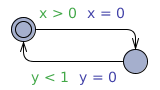
\includegraphics[scale=.5]{robust.png}
          \caption{Un automate temporisé.}
        \end{figure}

         \begin{block}{{\footnotesize\cite{alur94}} Automates temporisés}
           \begin{itemize}
             \item Automates finis étendus par des horloges 
             \item Contraintes temporelles sur les horloges \hfill $x \leq c$ \\
               \small avec $x$ une horloge, $c$ une constante
           \end{itemize}
         \end{block}

         \pause
         \begin{block}{Robustesse}
           \begin{itemize}
           \item Qualifie un modèle vis-à-vis de son implémentabilité
             \begin{itemize}
               \item Écart constaté à l'implémentation
               \item Conservation des propriétés du modèle
             \end{itemize}
           \end{itemize}
         \end{block}
       \end{frame}

    \subsection{Production scientifique}
      \begin{frame}
        \frametitle{\secname}
        \framesubtitle{\subsecname}
              
        \begin{figure}
          \centering
          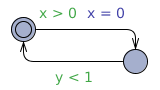
\includegraphics[scale=.5]{non-robust.png}
          \caption{Un automate temporisé non-robuste.}
        \end{figure}

        \vspace{1em}\pause
        \begin{block}{{\footnotesize\cite{sankur14}} {\it TA Shrinking}}
          \small
          Une contrainte temporelle réduite \hfill $x \leq c - \Delta$ \\
          avec $\Delta > 0$ un paramètre
        \end{block}

        \vspace{1em}\pause
        \begin{block}{{\footnotesize\cite{jovanovic14}} {\it Parametric TA}}
          \small
          Une contrainte temporelle paramétrée \hfill $x \leq p$ \\
          avec $p$ un paramètre
        \end{block}
        \vspace{3em}        
      \end{frame}

    \subsection{Réalisation d'un démonstrateur}
      \begin{frame}
        \frametitle{\secname}
        \framesubtitle{\subsecname}

        \small
        \begin{block}{Objectifs}
          \begin{itemize}
            \item Étude de cas sur la robustesse des modèles temporisés
            \item Système cyber-physique, temps réel, communicant et concurrent
            \item Réutilisable dans le cadre d'autres projets
          \end{itemize}
        \end{block}
      \end{frame}

    \subsection{Travail attendu}
      \begin{frame}
        \frametitle{\secname}
        \framesubtitle{\subsecname}

        % TODO Aspect ingénierie, aspect recherche
        \begin{block}{Implémentation}
          \begin{itemize}
            \item Implémentation matérielle et logicielle
          \end{itemize}
        \end{block}

        \pause
        \begin{block}{Modélisation}
          \begin{itemize}
            \item Modélisation architecturale
            \item Modélisation comportementale
          \end{itemize}
        \end{block}

        \pause
        \begin{block}{Analyse de robustesse}
          \begin{itemize}
            \item Mise en \oe uvre des résultats théoriques
            \item Constatations concrètes sur l'implémentation
          \end{itemize}
        \end{block}
      \end{frame}

  \section{Réalisation d'une implémentation}
    \subsection{Spécification du démonstrateur}
      \begin{frame}
        \frametitle{\secname}
        \framesubtitle{\subsecname}
       
        \vfill
        \begin{figure}
          \centering
          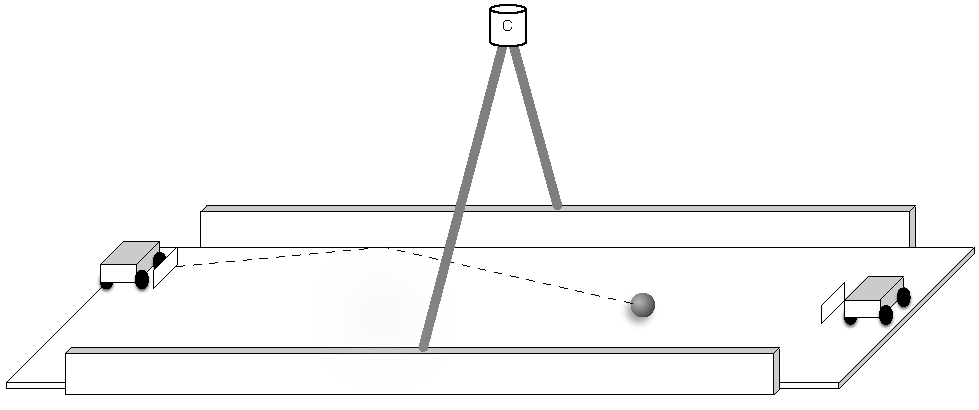
\includegraphics[height=.35\textheight]{spec-demo1.pdf} \\
          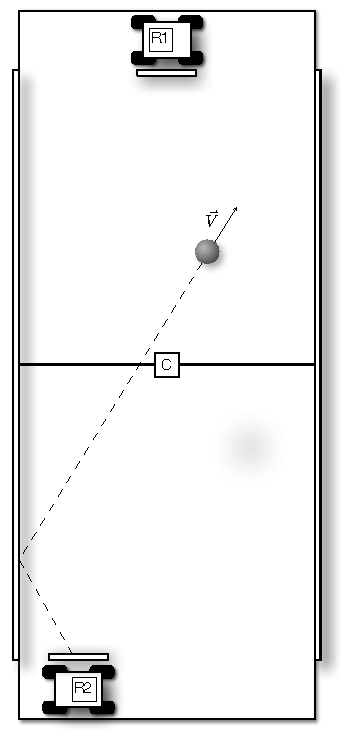
\includegraphics[angle=270, totalheight=.35\textheight]{spec-demo2.pdf}
          \caption{{\footnotesize\cite{bechennec12}} Schémas de la spécification
            du démonstrateur.}
        \end{figure}
      \end{frame}

    \subsection{Implémentation matérielle et logicielle}
      \begin{frame}
        \frametitle{\secname}
        \framesubtitle{\subsecname}

        \begin{block}{Moyens}
          \begin{itemize}
            \item Base matérielle en Lego Technics
              \begin{itemize}
                \item Lego Mindstorms NXT, ARM7 32bit
                \item Arduino Uno, AVR 8bit, bus I2C
                \item CMUcam4, bus UART
              \end{itemize}
            \pause
            \item {\footnotesize\cite{bechennec06}} Trampoline, système
              d'exploitation temps réel
              \begin{itemize}
                \item Développé par l'équipe Systèmes Temps Réel de l'IRCCyN
                \item Conforme aux standards OSEK/VDX et AUTOSAR
              \end{itemize}
          \end{itemize}
        \end{block}

        \pause
        \begin{block}{Résultats}
          \begin{itemize}
            \item Implémentation fonctionnelle
              \begin{itemize}
                \item Différents prototypes matériels
                \item Intervention dans le code système et applicatif 
              \end{itemize}
            \item Implémentation validée en réunion de travail
          \end{itemize}
        \end{block}
      \end{frame}

      \begin{frame}
        \frametitle{\secname}

        \begin{figure}
          \centering
          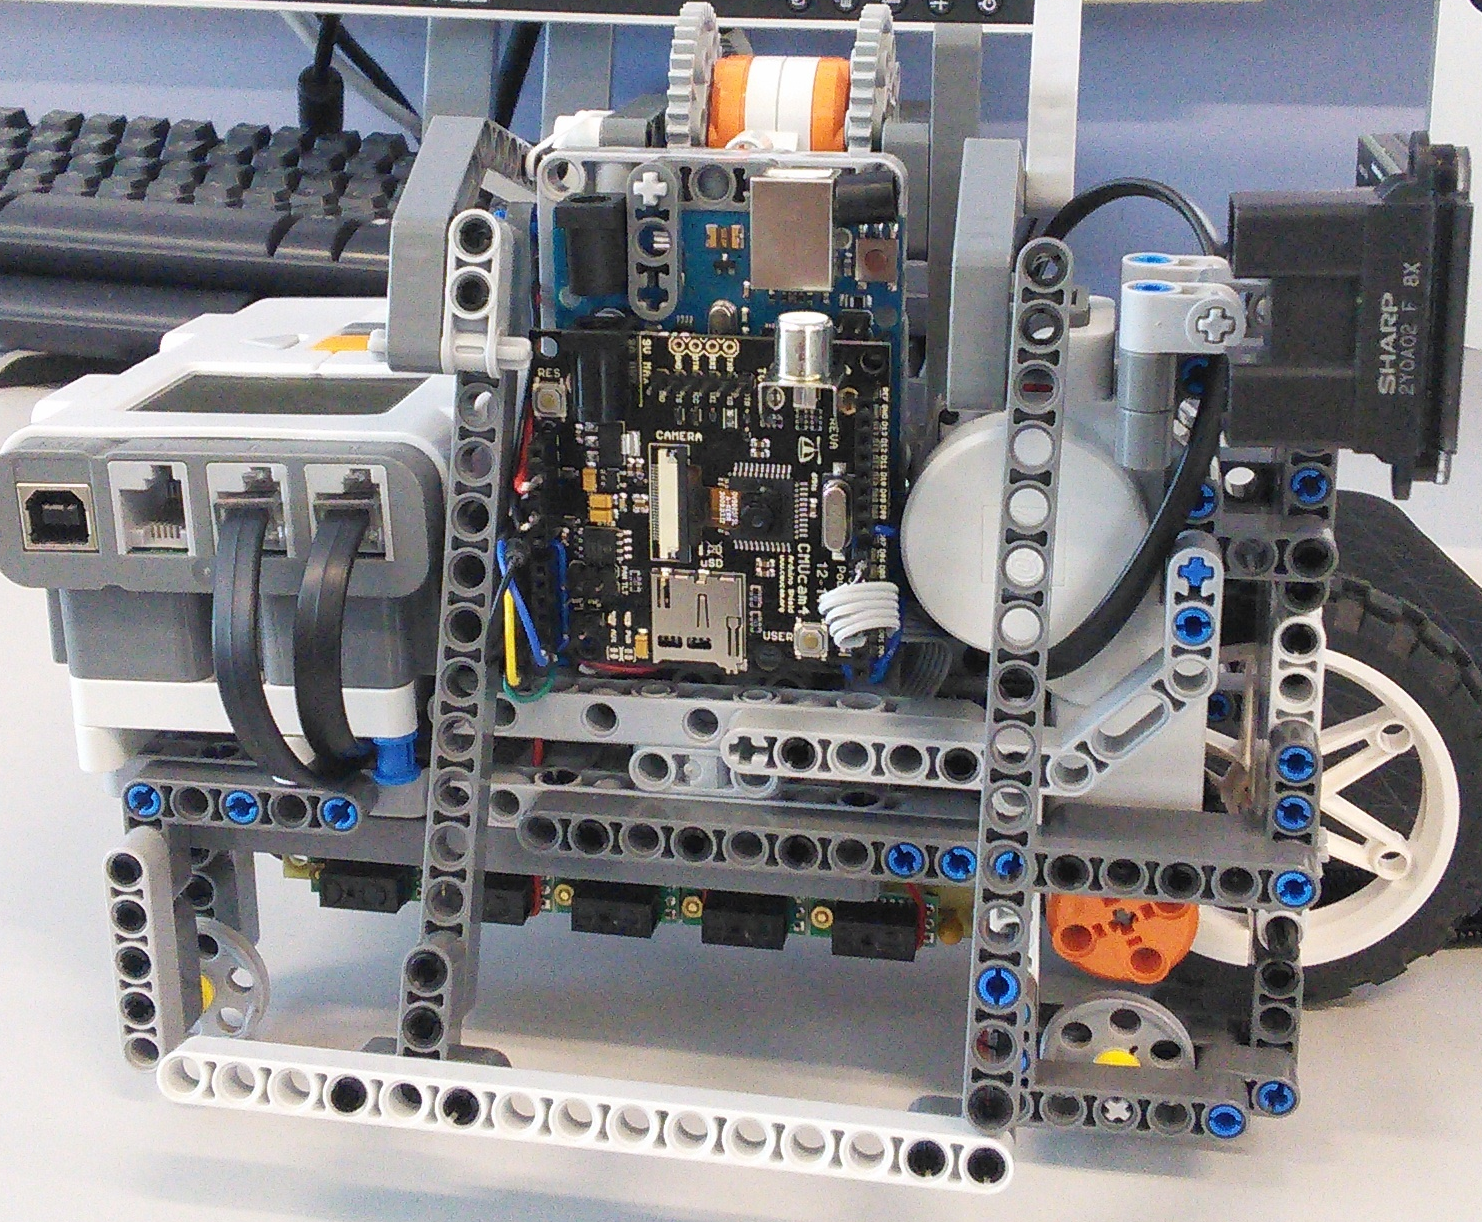
\includegraphics[width=0.8\textwidth]{impl-robot.png}
          \caption{Implémentation matérielle.}
        \end{figure}
      \end{frame}

  \section{Réalisation d'un modéle}
    \subsection{Modélisation architecturale}
      \begin{frame}
        \frametitle{\secname}        
        \framesubtitle{\subsecname}
 
        \begin{block}{Objectifs}
          \begin{itemize}
            \item Introduction au fonctionnement du démonstrateur 
            \item Documentation pour réutilisation du démonstrateur
            %\item Vocabulaire commun
          \end{itemize}
        \end{block}
          
        \pause
        \begin{block}{Moyens}
          \begin{itemize}
            \item {\footnotesize\cite{aadl}} {\it Architecture Analysis \&
              Design Language} (AADL)
              \begin{itemize}
                \item Sémantique adapté à l'embarqué temps réel
                \item Méthode de modélisation orientée langage
                \item Permettant la vérification et la génération
              \end{itemize}
          \end{itemize}
        \end{block}

        \pause
        \begin{block}{Résultats}
          \begin{itemize}
            \item Modélisation complète de l'architecture robot
              \begin{itemize}
                \item Deux modélisations : première et seconde spécification
                \item 100 composants, 74 connections
              \end{itemize}
            \item Modélisation validée en réunion de travail
            %\item Mise à disposition pour divers projets
          \end{itemize}
        \end{block}
      \end{frame}

%      \begin{frame}
%        \frametitle{\secname}        
%        \framesubtitle{\subsecname}
%        
%        \begin{figure}
%          \centering
%          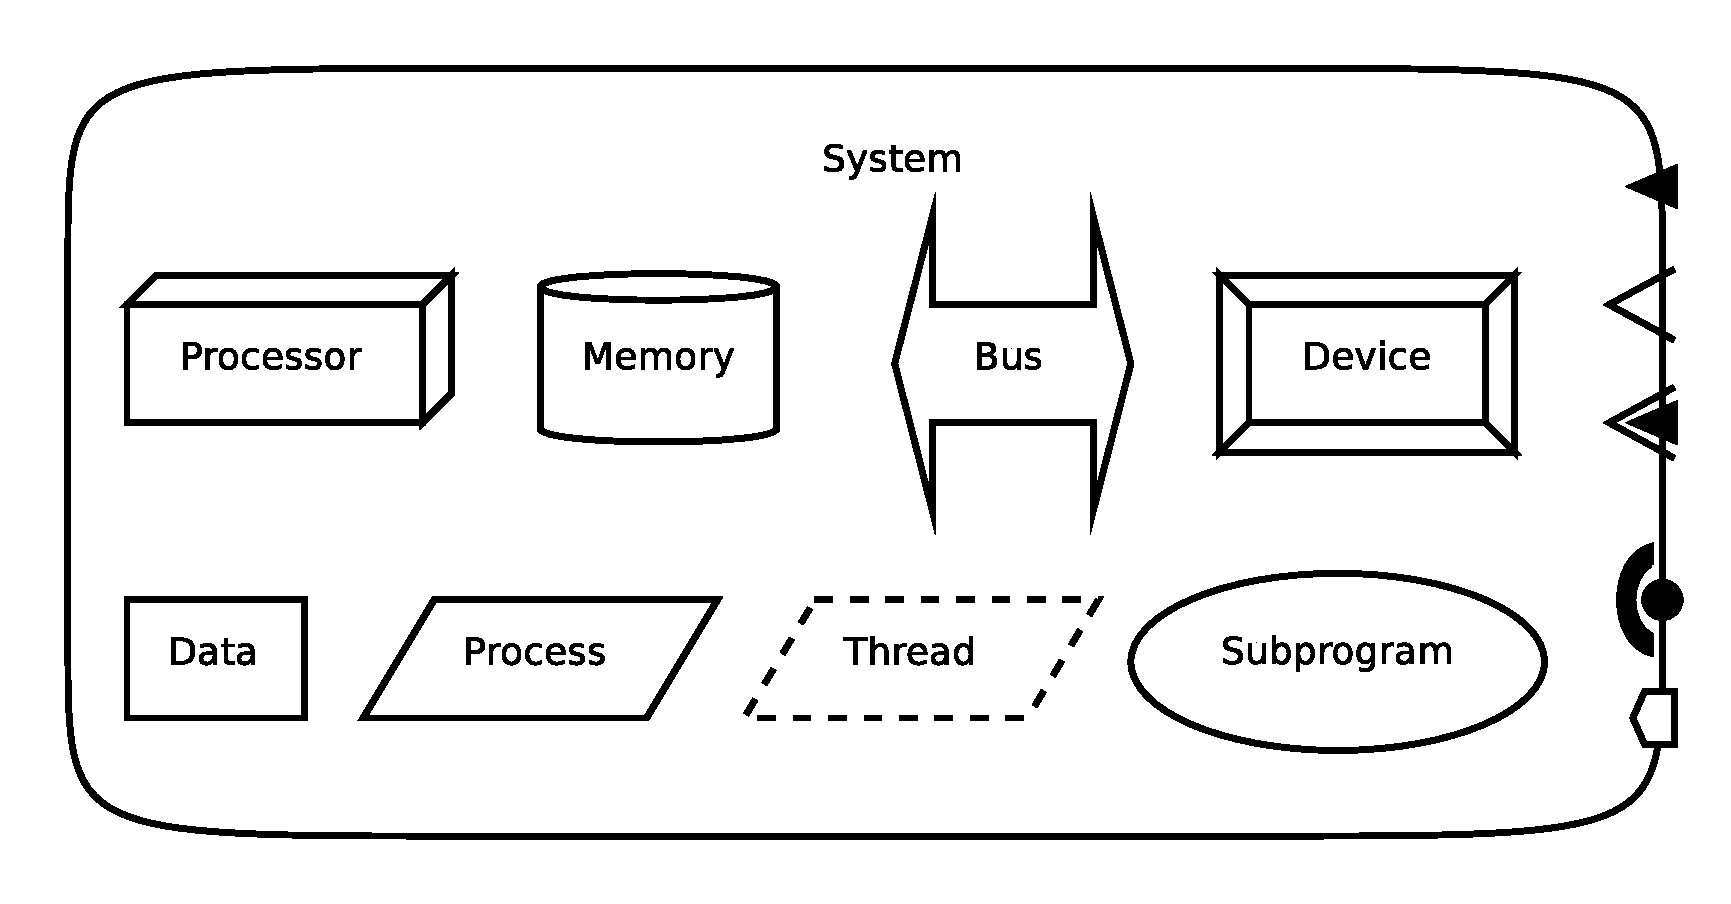
\includegraphics[width=.8\textwidth]{aadl-memo.pdf}
%          \caption{Introduction à AADL.}
%        \end{figure}
%      \end{frame}

%      \begin{frame}
%        \frametitle{\subsecname}        
%        \framesubtitle{Modélisation structurelle}
%
%        \begin{figure}
%          \centering
%          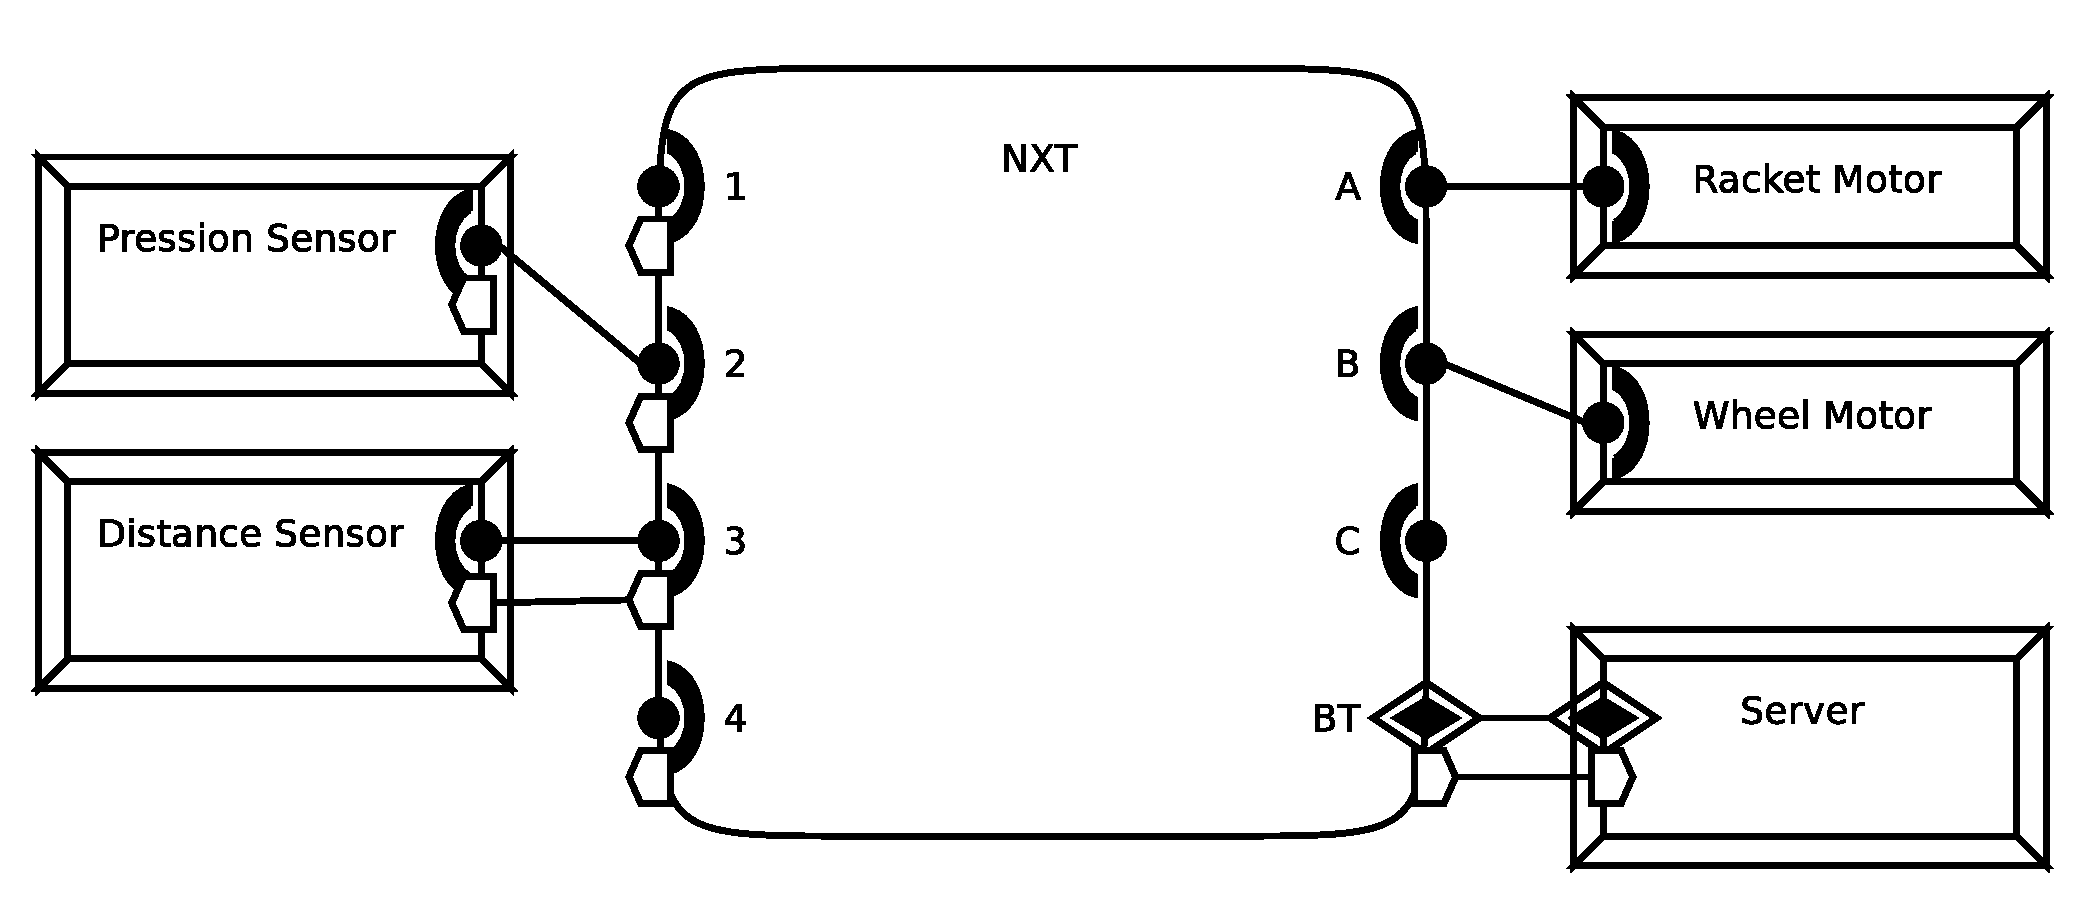
\includegraphics[width=.8\textwidth]{aadl-robot1.pdf}
%          \caption{Vue générale du robot.}
%        \end{figure}
%      \end{frame}

%      \begin{frame}
%        \frametitle{\subsecname}        
%        \framesubtitle{Modélisation structurelle}
%
%        \begin{figure}
%          \centering
%          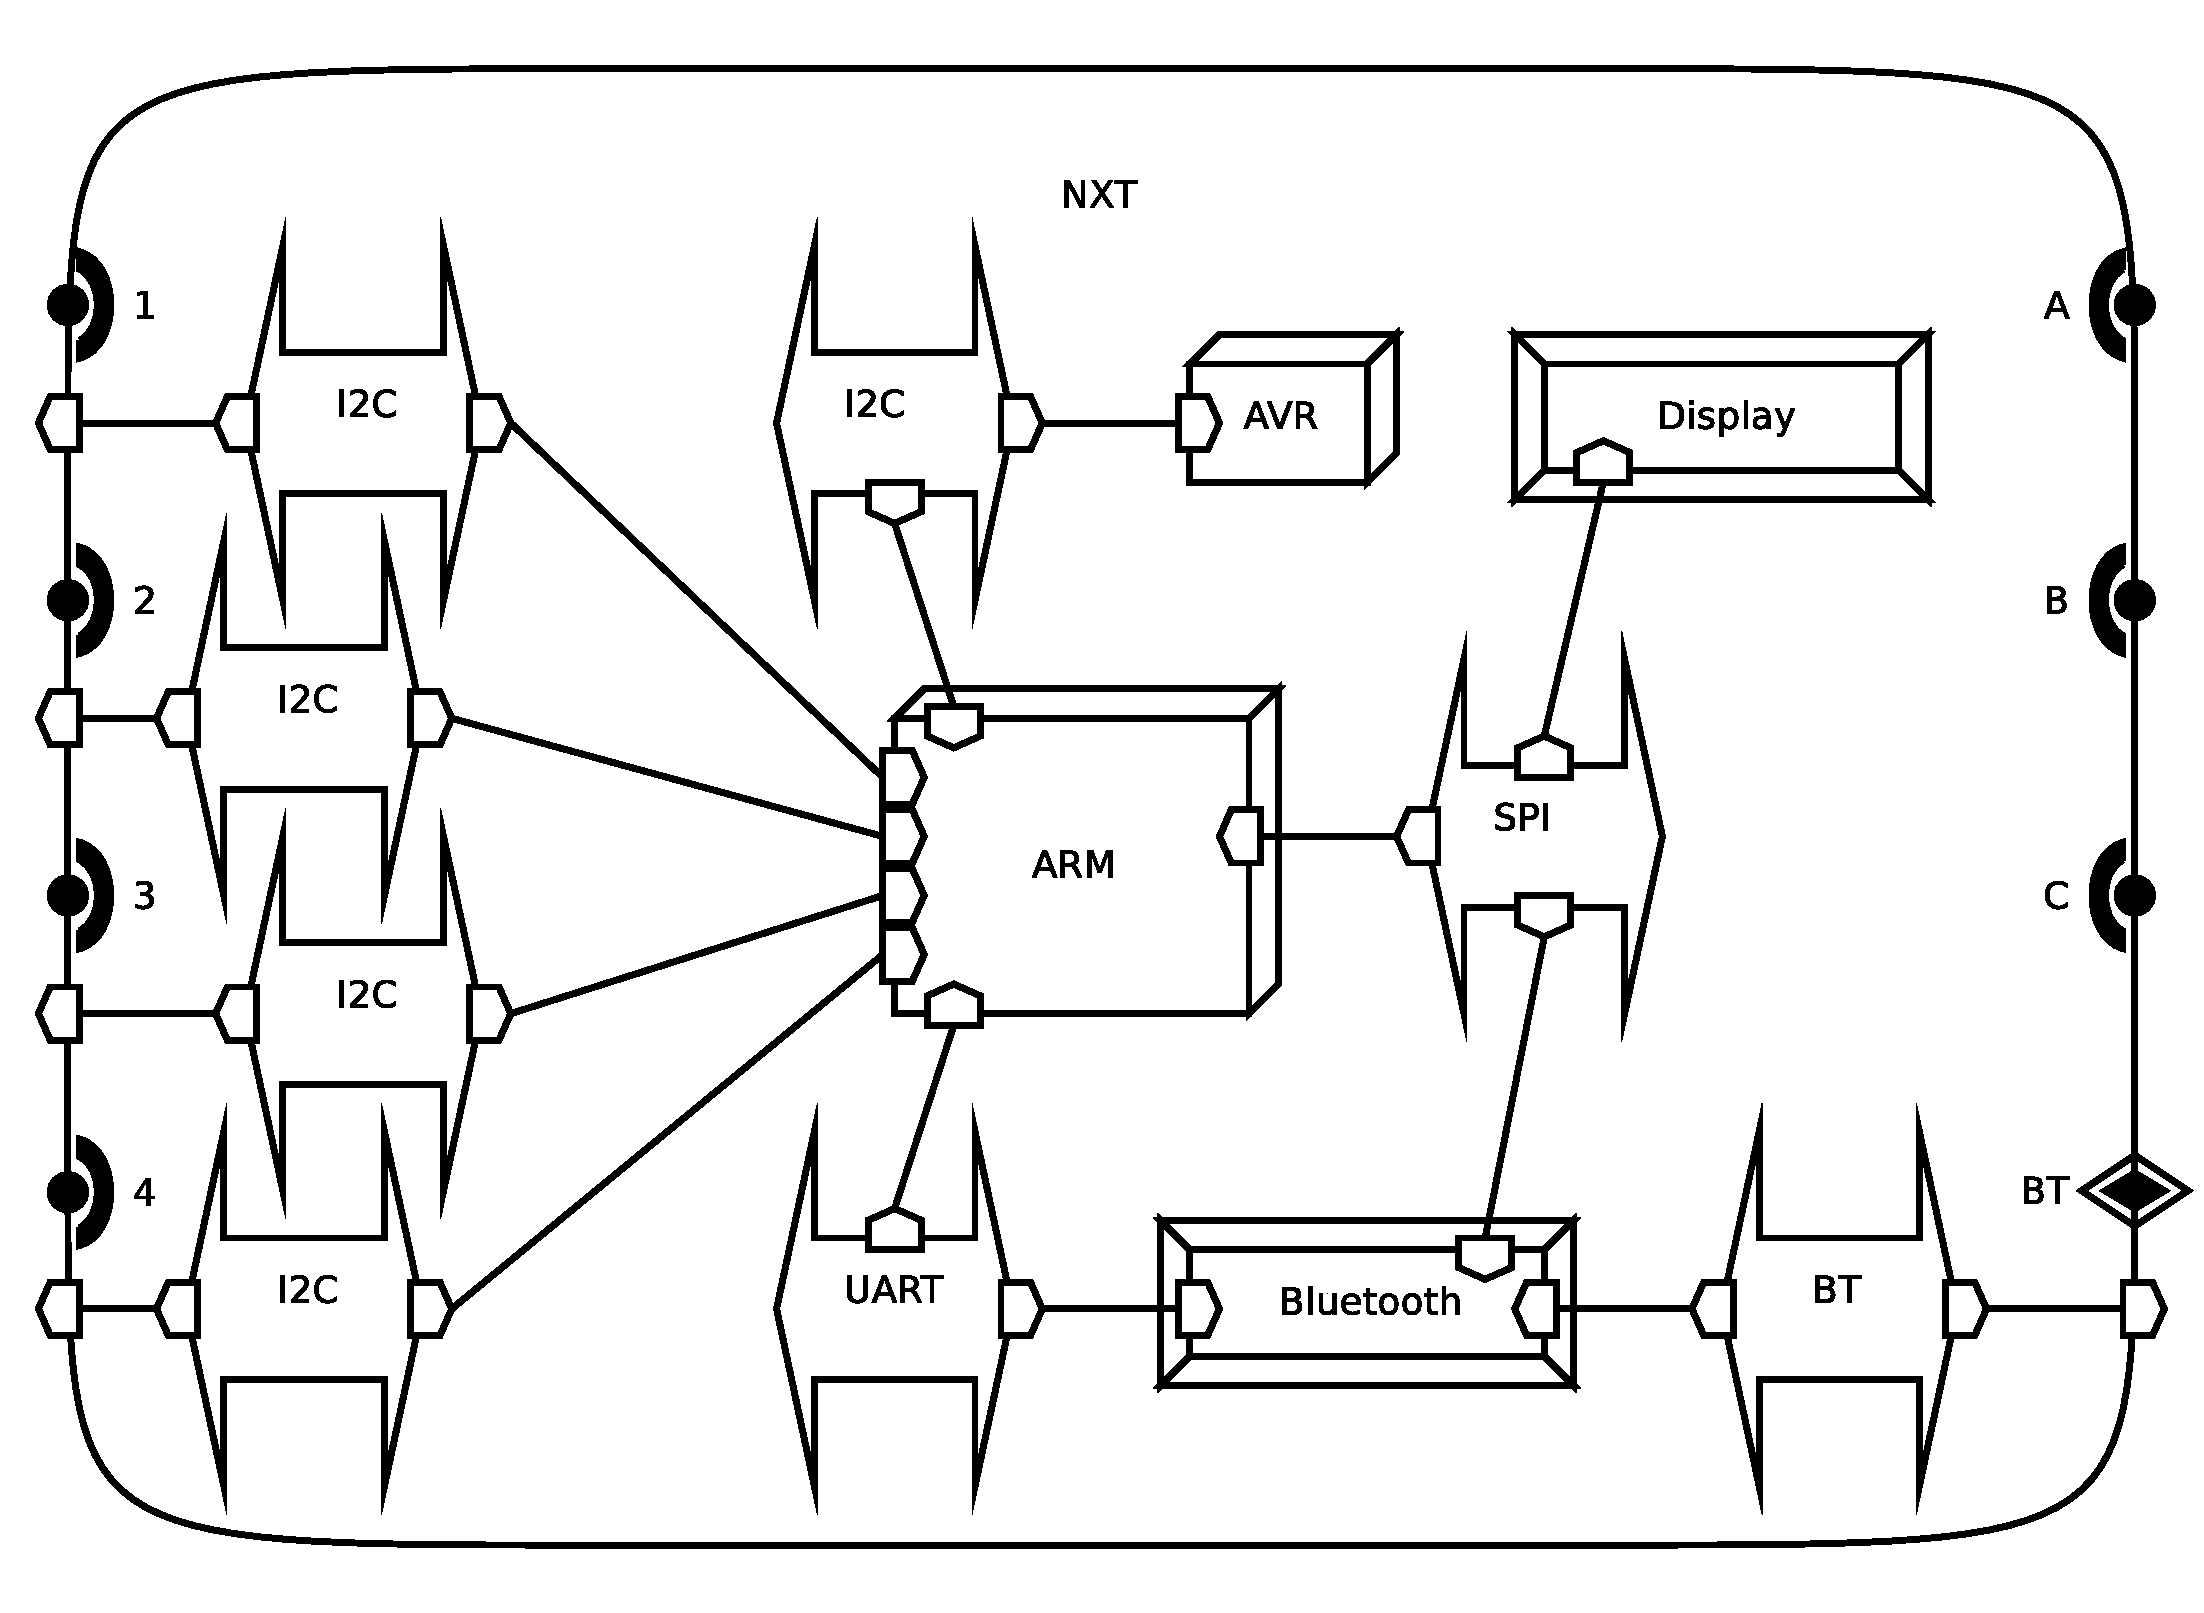
\includegraphics[width=.8\textwidth]{aadl-nxt1h.pdf}
%          \caption{Modèle matériel du NXT.}
%        \end{figure}
%      \end{frame}

%      \begin{frame}
%        \frametitle{\subsecname}        
%        \framesubtitle{Modélisation structurelle}
%
%        \begin{figure}
%          \centering
%          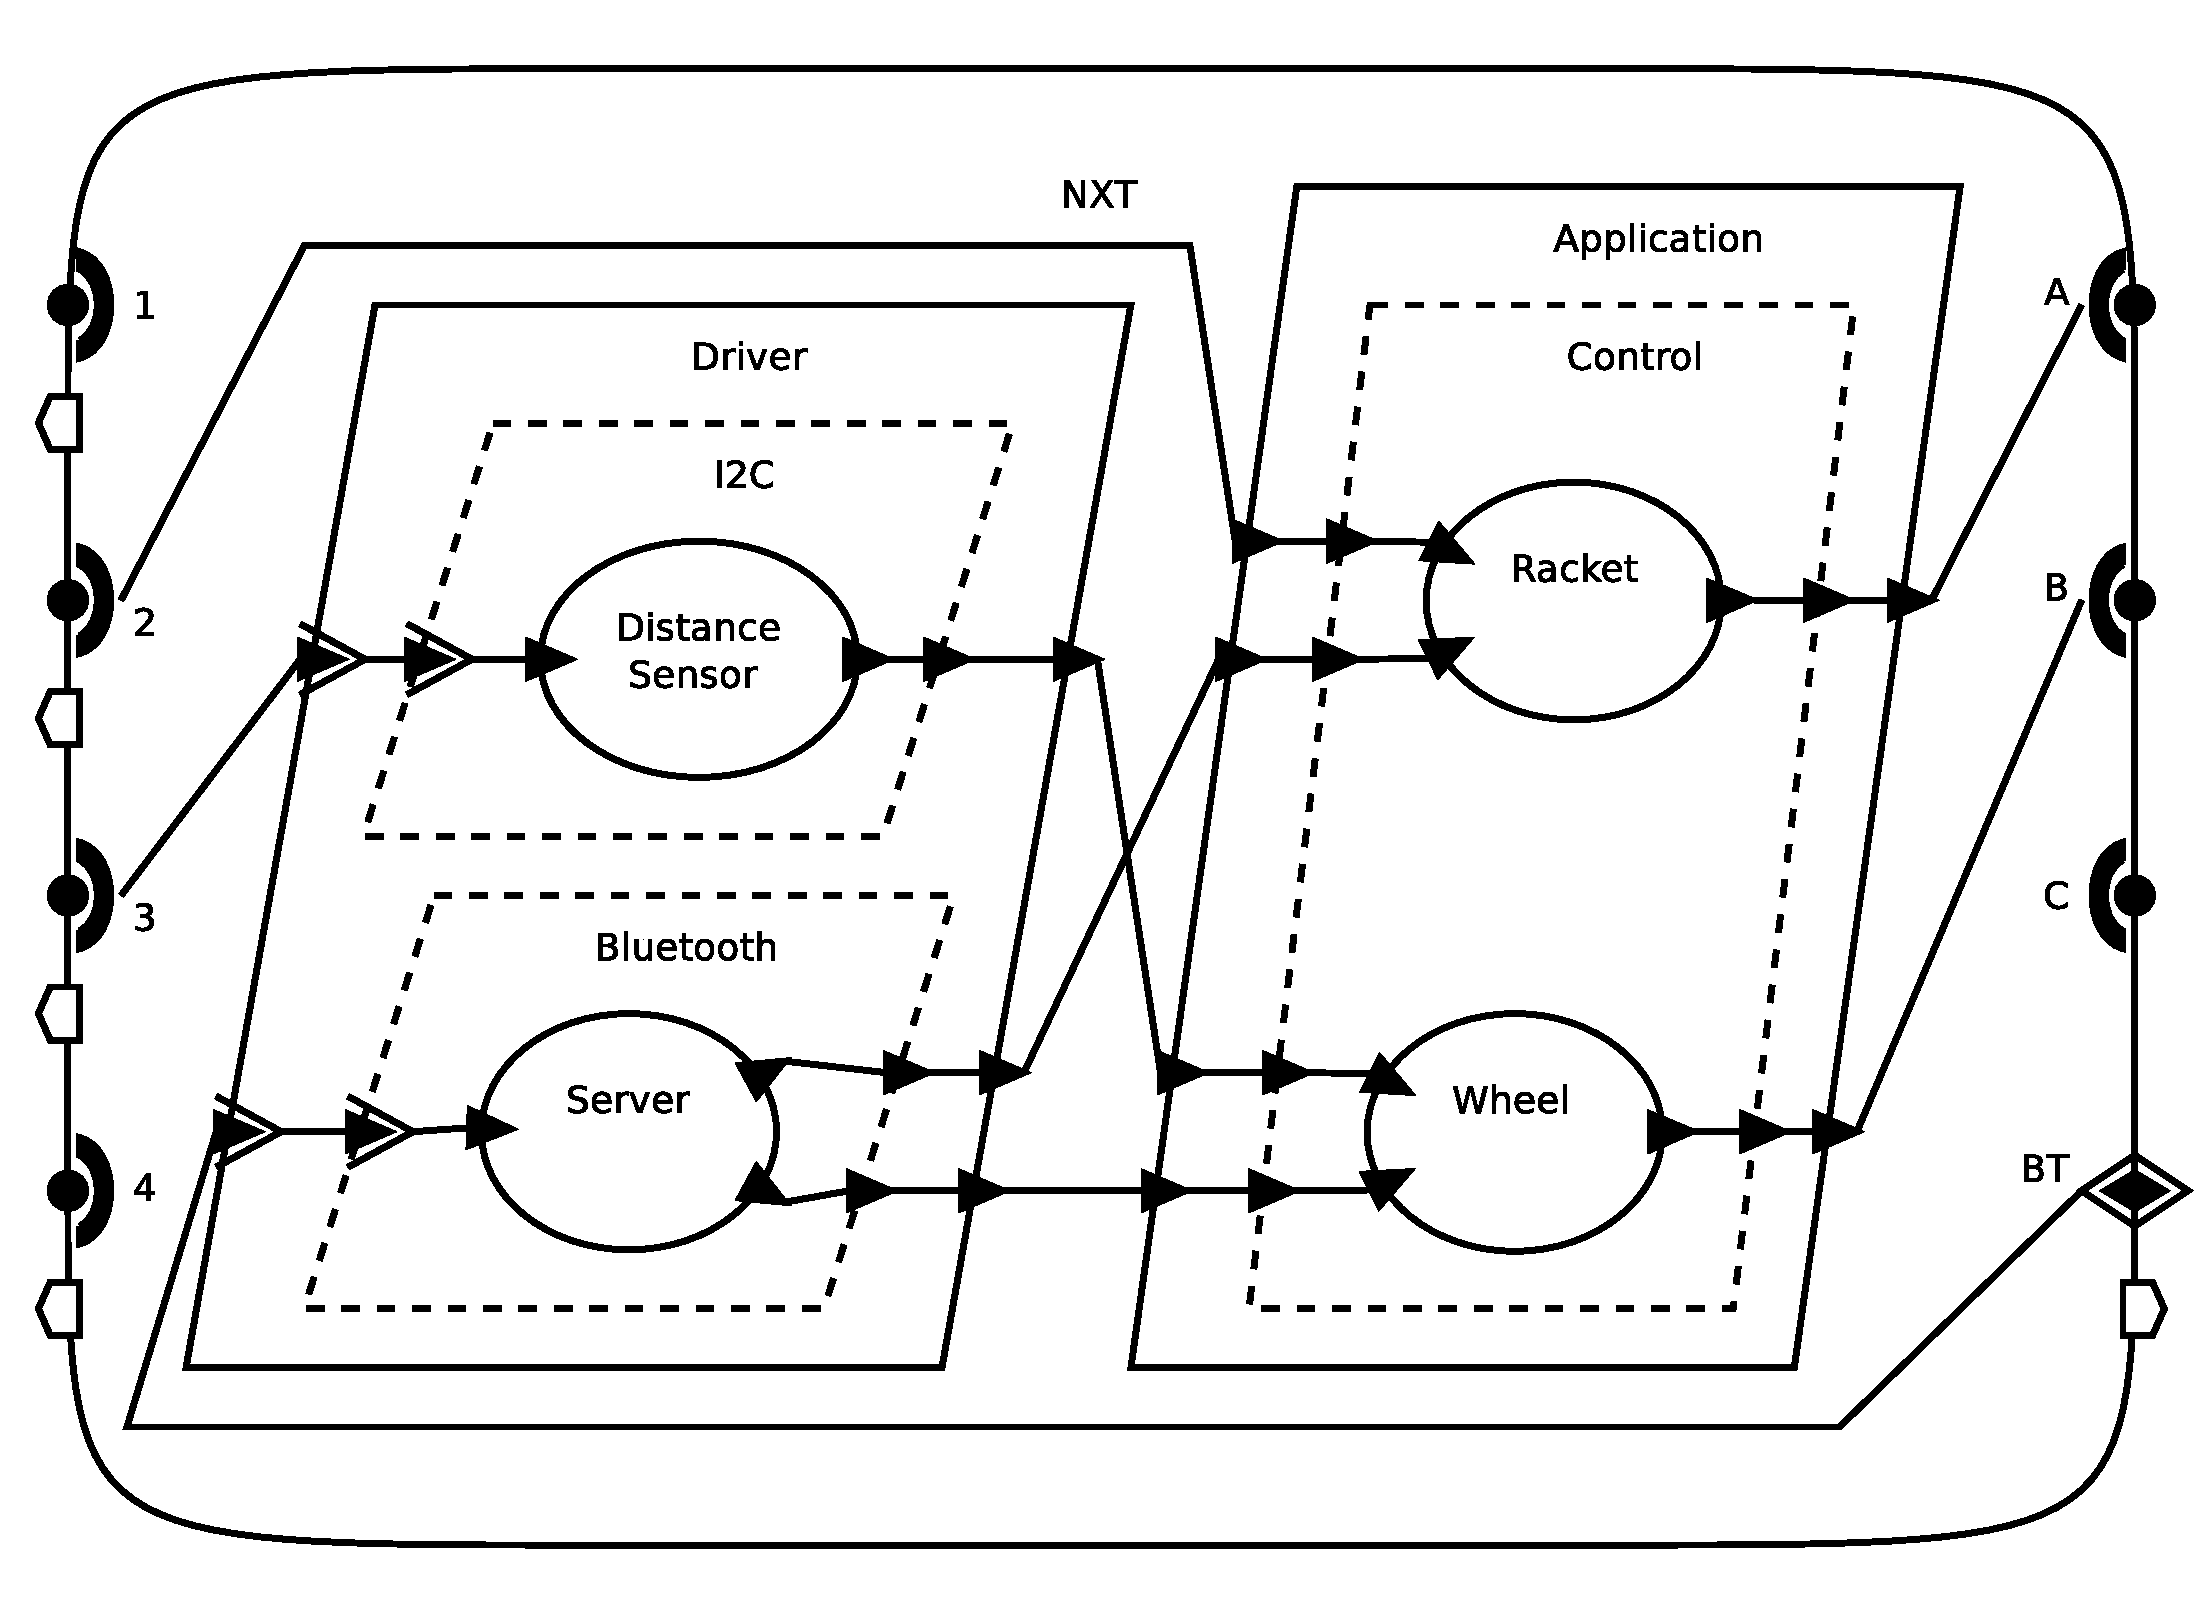
\includegraphics[width=.8\textwidth]{aadl-nxt1s.pdf}
%          \caption{Modèle logiciel du NXT.}
%        \end{figure}
%      \end{frame}

%      \begin{frame}
%        \frametitle{\subsecname}
%        \framesubtitle{Modification de la spécification}
%
%        \begin{block}{Contraintes techniques}
%          \begin{itemize}
%            \item Problème de latences trop importantes
%            \item Ajout d'une caméra embarquée et de capteurs de présence
%            \item L'implémentation a fait l'objet d'un autre stage
%          \end{itemize}
%        \end{block}
%      \end{frame}

      \begin{frame}
        \frametitle{\secname}        
        \framesubtitle{\subsecname}

        \begin{figure}
          \centering
          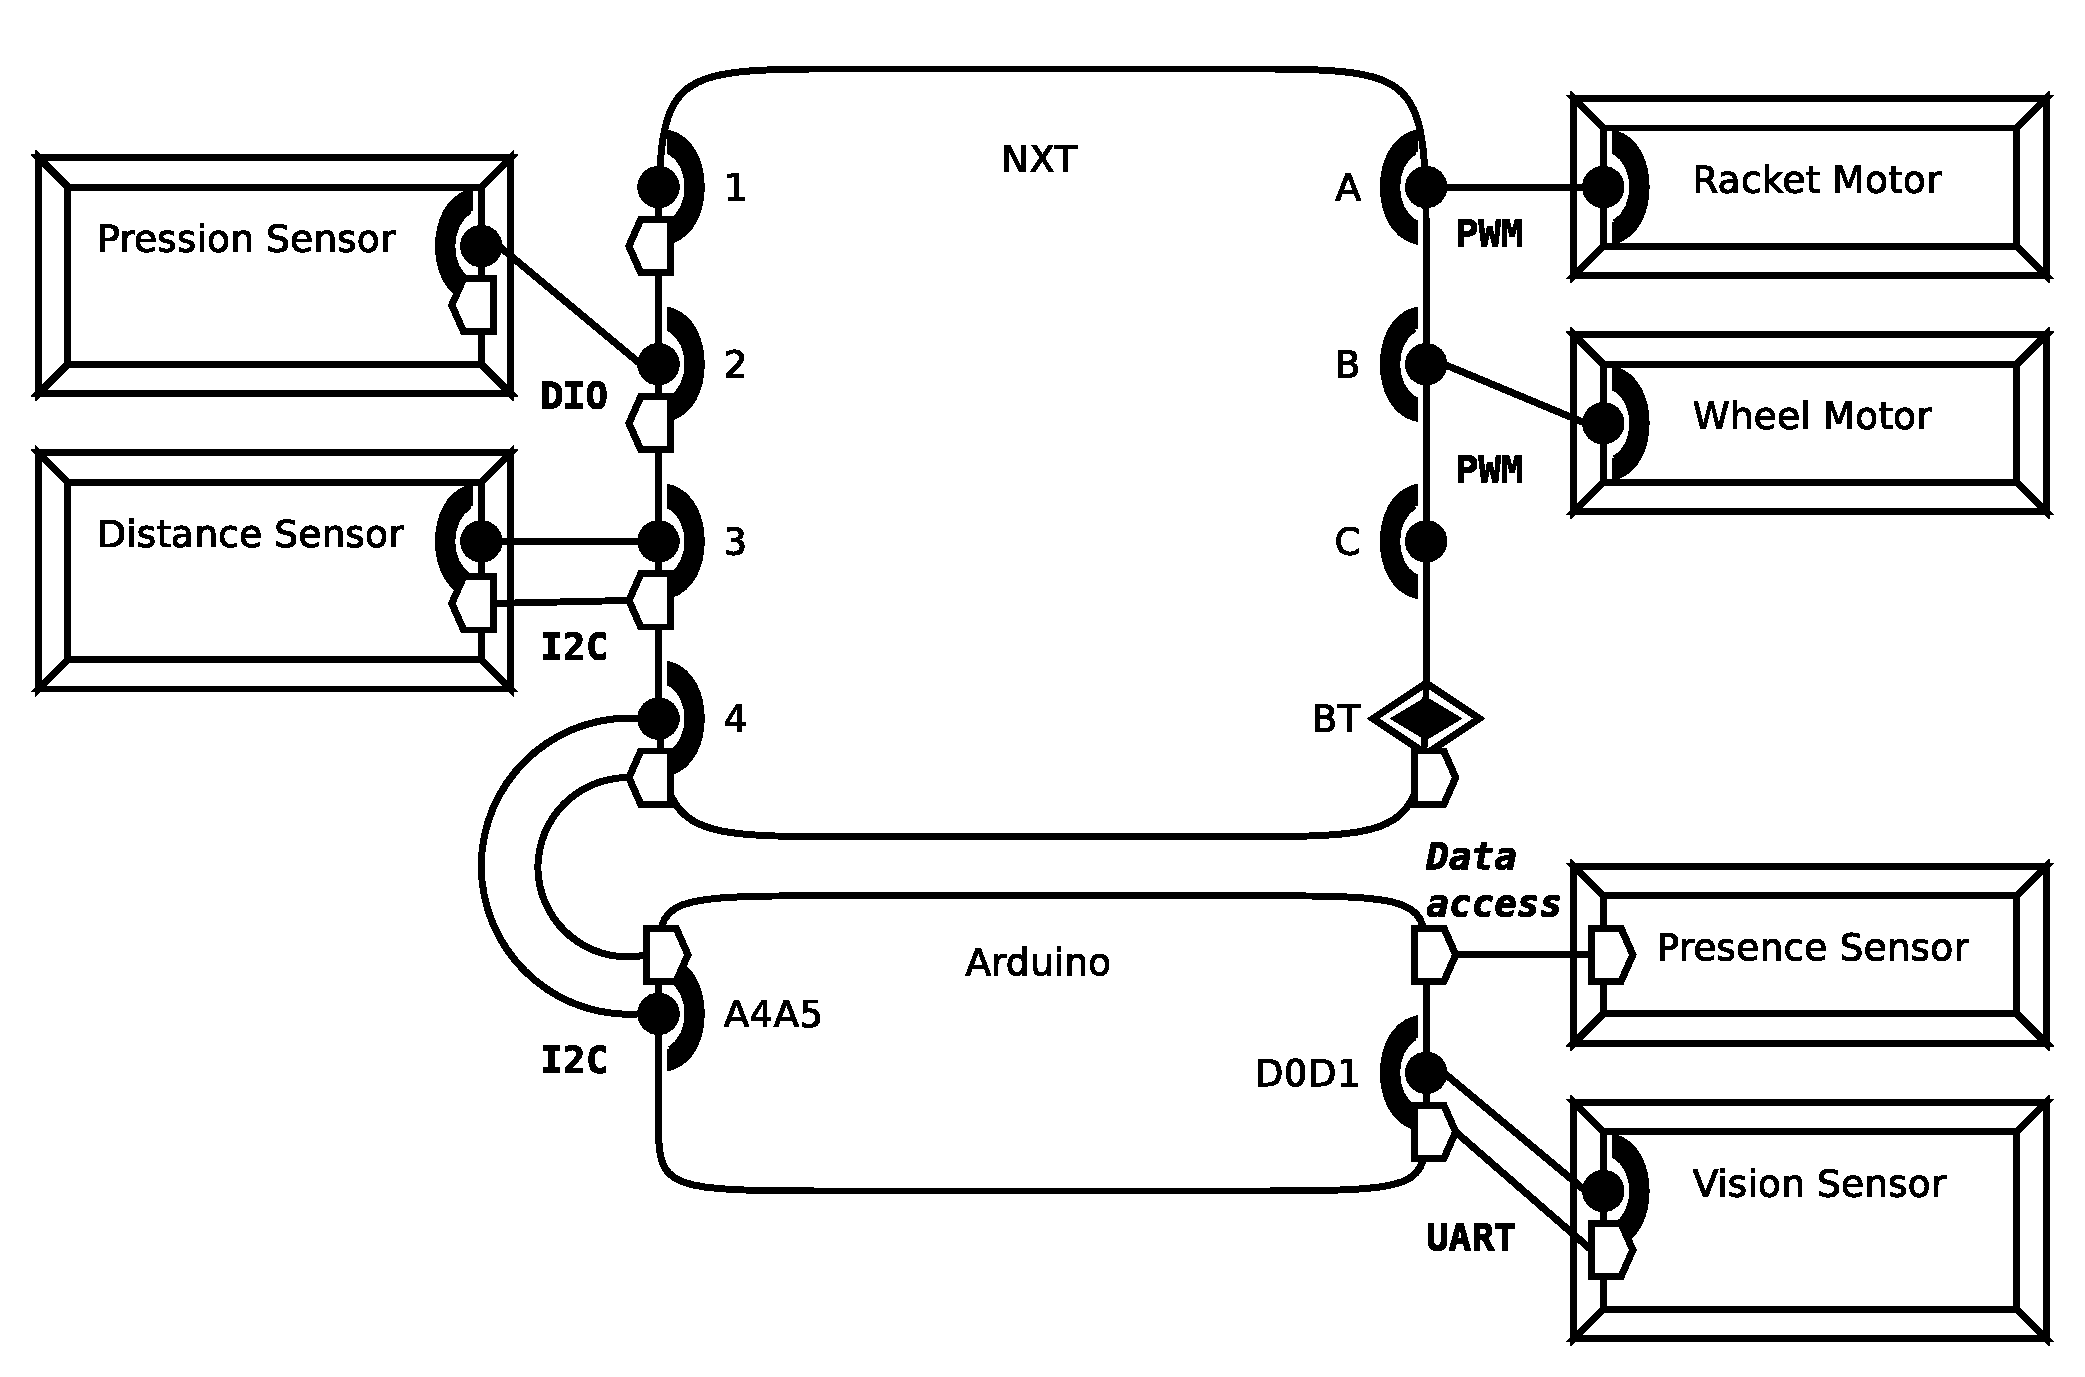
\includegraphics[width=.8\textwidth]{aadl-robot2.pdf}
          \caption{Modèle AADL du robot.}
        \end{figure}
      \end{frame}

%      \begin{frame}
%        \frametitle{\secname}        
%        \framesubtitle{\subsecname}
%
%        \begin{figure}
%          \centering
%          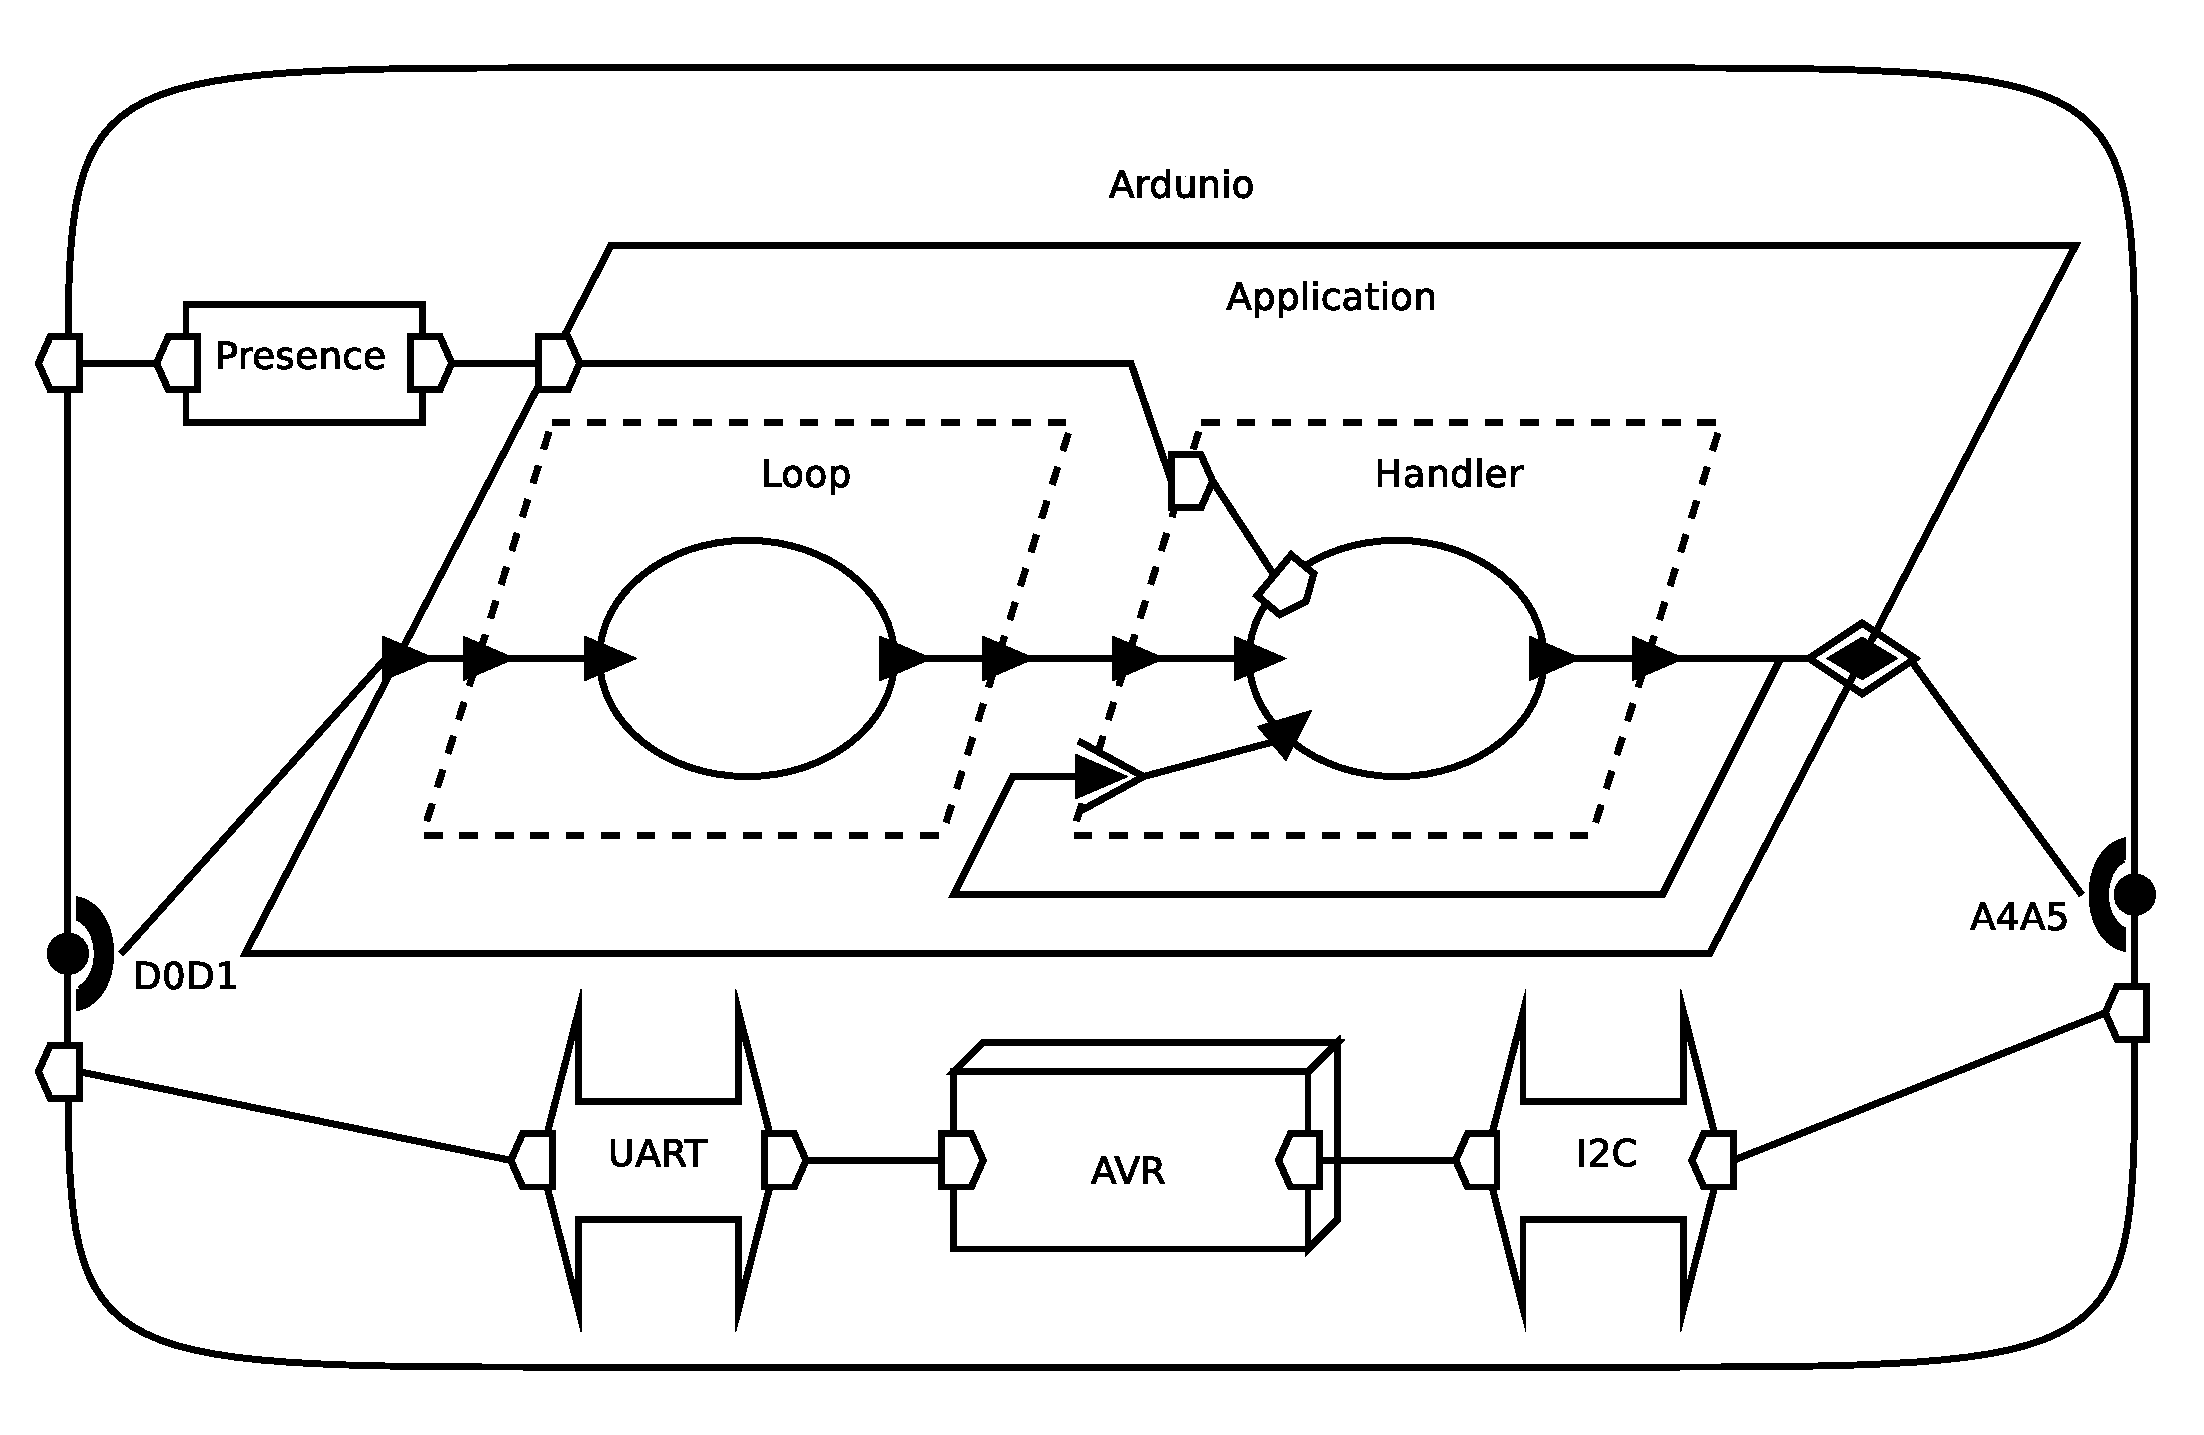
\includegraphics[width=.8\textwidth]{aadl-arduino.pdf}
%          \caption{Modèle de l'Arduino.}
%        \end{figure}
%      \end{frame}

      \begin{frame}
        \frametitle{\secname}        
        \framesubtitle{\subsecname}

        \begin{figure}
          \centering
          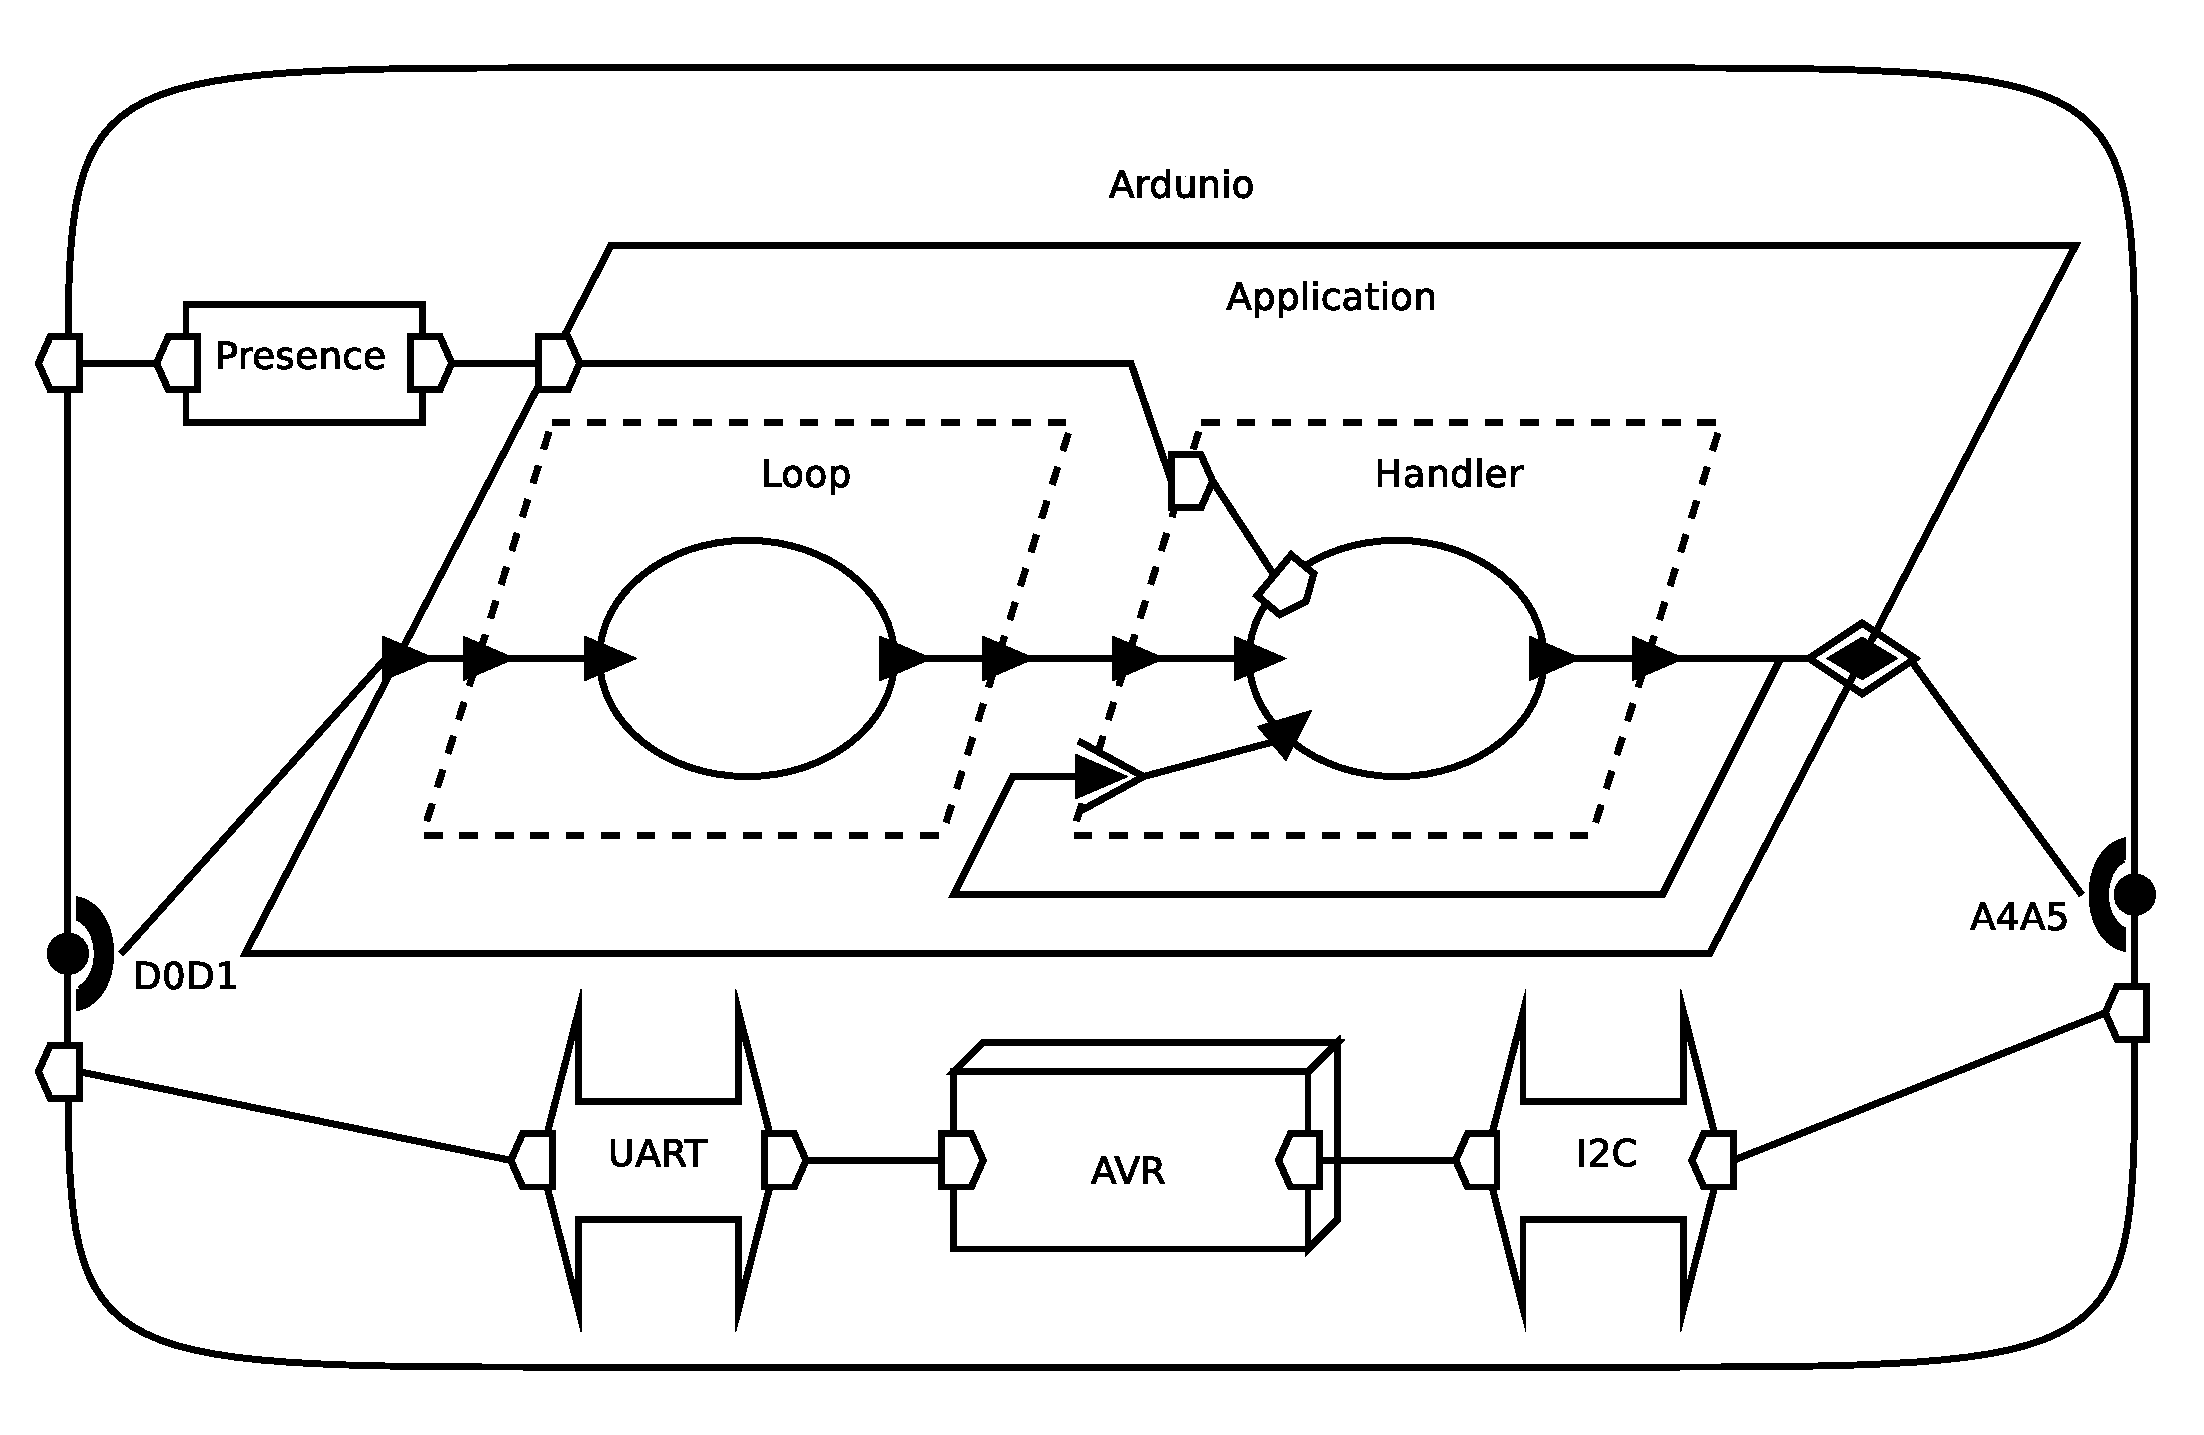
\includegraphics[width=.8\textwidth]{aadl-arduino.pdf}
          \caption{Modèle AADL de l'Arduino}
        \end{figure}
      \end{frame}

    \subsection{Modélisation comportementale}
      \begin{frame}
        \frametitle{\secname}
        \framesubtitle{\subsecname}

        \begin{block}{Objectifs}
          \begin{itemize}
            \item Support pour la vérification du démonstrateur
            \item Support pour l'implémentation du démonstrateur
          \end{itemize}
        \end{block}
        \pause

        \begin{block}{Moyens}
          \begin{itemize}
            \item {\footnotesize\cite{larsen97}} UPPAAL, environnement de
              modélisation de TA
              \begin{itemize}
                \item Adapté aux résultats de recherche à mettre en \oe uvre  
                \item Interface graphique pour la modélisation
                \item Outils de simulation et de vérification
              \end{itemize}
          \end{itemize}
        \end{block}

        \pause
        \begin{block}{Résultats}
          \begin{itemize}
            \item Modélisation partielle du comportement du robot
              \begin{itemize}
                \item Deux modélisations : pragmatique et idéale
                \item 8 TA, 33 états, 10 horloges, 13 {\it channels}
              \end{itemize}
            \item Validation du modèle par vérification de propriétés
          \end{itemize}
        \end{block}
      \end{frame}

%      \begin{frame}[shrink]
%        \frametitle{\subsecname}
%        \framesubtitle{Modélisation fonctionnelle}
%
%        \begin{figure}
%          \centering
%          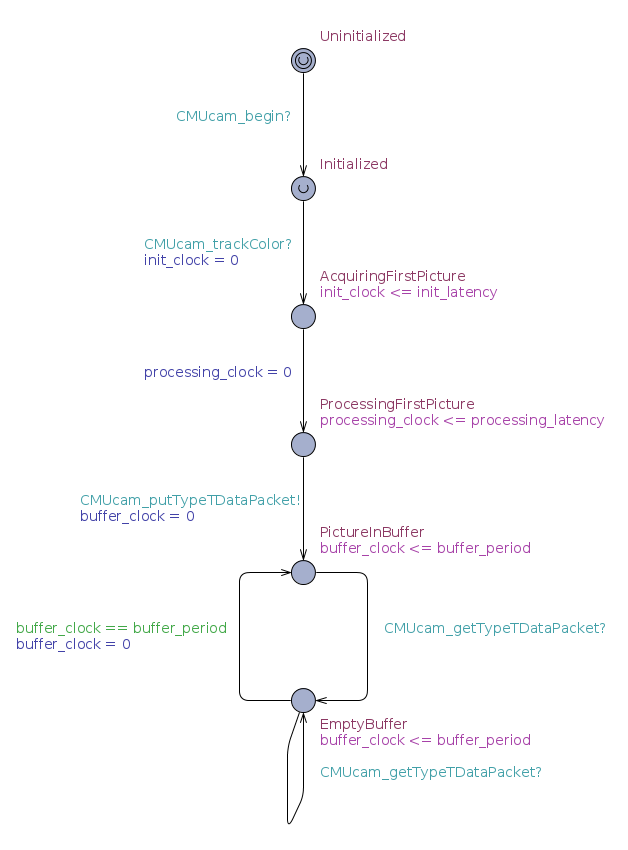
\includegraphics[width=.8\textwidth]{uppaal-camera.png}
%          \caption{Modèle de la caméra.}
%        \end{figure}
%      \end{frame}

%      \begin{frame}[shrink]
%        \frametitle{\subsecname}
%        \framesubtitle{Modélisation fonctionnelle}
%
%        \begin{figure}
%          \centering
%          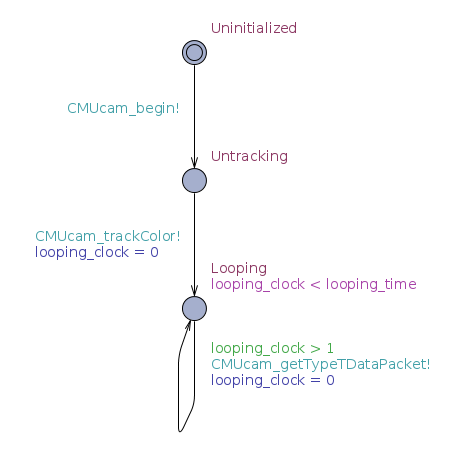
\includegraphics[width=.8\textwidth]{uppaal-loop.png}
%          \caption{Modèle de la {\it loop} Arduino.}
%        \end{figure}
%      \end{frame}

%      \begin{frame}[shrink]
%        \frametitle{\subsecname}
%        \framesubtitle{Modélisation fonctionnelle}
%
%        \begin{figure}
%          \centering
%          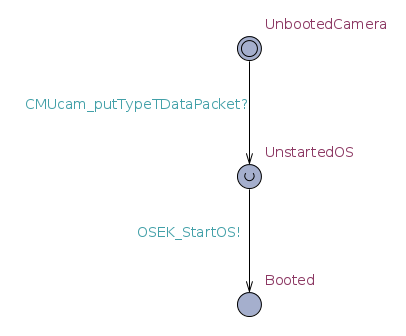
\includegraphics[width=.8\textwidth]{uppaal-boot.png}
%          \caption{Modèle de démarrage du NXT.}
%        \end{figure}
%      \end{frame}

      \begin{frame}
        \frametitle{\secname}
        \framesubtitle{\subsecname}

        \begin{figure}
          \centering
          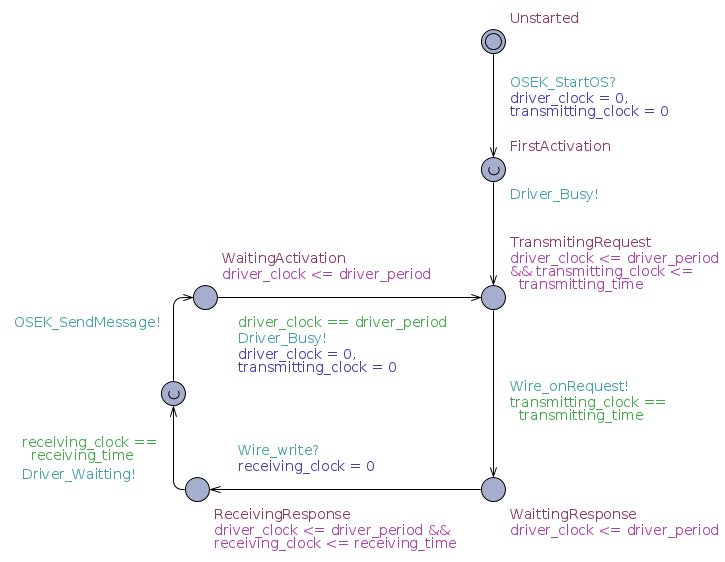
\includegraphics[scale=.33]{uppaal-driver.png}
          \caption{Modèle du pilote I2C du NXT.}
        \end{figure}
      \end{frame}

%      \begin{frame}[b]
%        \frametitle{\secname}
%        \framesubtitle{\subsecname}
%
%        \begin{figure}[b]
%          \centering
%          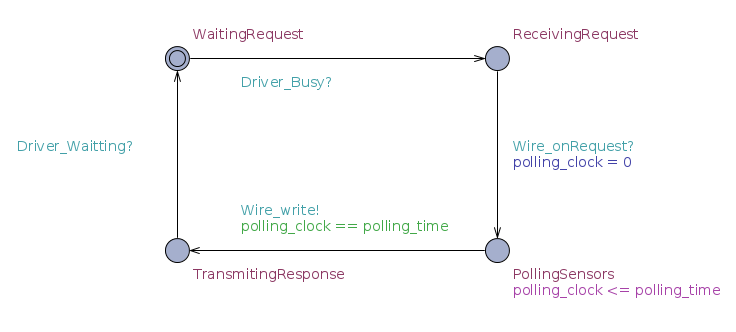
\includegraphics[scale=.33]{uppaal-handler.png}
%          \caption{Modèle du {\it handler} Arduino.}
%        \end{figure}
%      \end{frame}

%      \begin{frame}
%        \frametitle{\secname}
%        \framesubtitle{\subsecname}
%
%        \begin{figure}
%          \centering
%          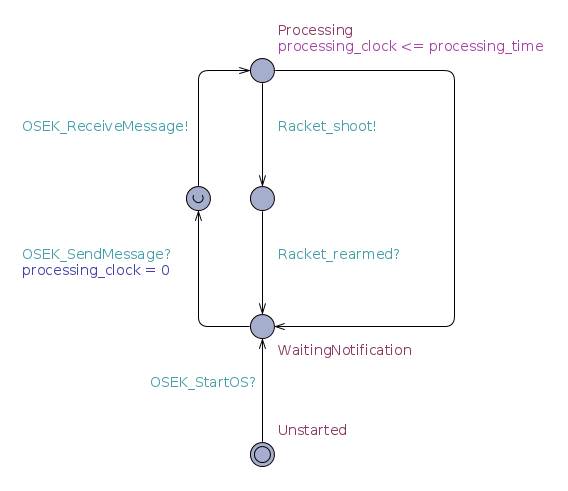
\includegraphics[width=.8\textwidth]{uppaal-task.png}
%          \caption{Modèle de la tâche du NXT.}
%        \end{figure}
%      \end{frame}

%      \begin{frame}[shrink]
%        \frametitle{\subsecname}
%        \framesubtitle{Modélisation fonctionnelle}
%
%        \begin{figure}
%          \centering
%          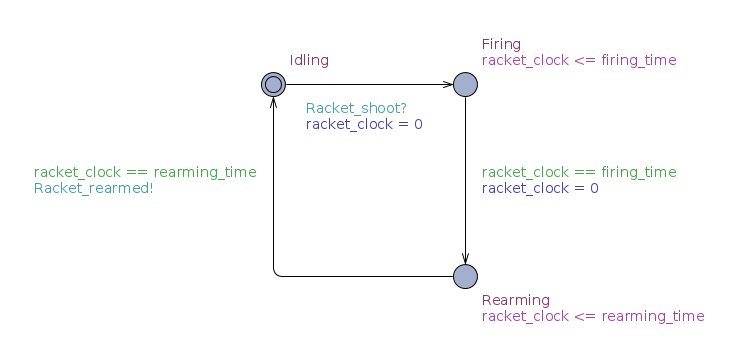
\includegraphics[width=.8\textwidth]{uppaal-racket.png}
%          \caption{Modèle de la raquette.}
%        \end{figure}
%      \end{frame}

  \section{Réalisation d'une analyse}
    \subsection{Vérification et synthèse de paramètres}
      \begin{frame}
        \frametitle{\secname}
        \framesubtitle{\subsecname}

        \begin{block}{Objectifs}
          \begin{itemize}
            \item Mise en \oe uvre des résultats de recherche
            \item Analyse de la robustesse du démonstrateur
          \end{itemize}
        \end{block}
        \pause

        \begin{block}{Moyens}
          \begin{itemize}
            \item {\footnotesize\cite{sankur13}} Shrinktech, approche par {\it
              TA Shrinking}
            \item {\footnotesize\cite{lime09}} Roméo, approche par {\it
              Parametrics TA}
              \begin{itemize}
                \item Développé par l'équipe Systèmes Temps Réel de l'IRCCyN
                \item Vérification de réseaux de Petri T-temporels
                \item {\footnotesize\cite{lime12}} Manipulation de {\it Clock
                  Transition Systems}
              \end{itemize}
          \end{itemize}
        \end{block}
      \end{frame}

      \begin{frame}
        \frametitle{\secname}
        \framesubtitle{\subsecname}
        
        \begin{block}{Vérification}
          \begin{itemize}
            \item Absence d'interblocage \\
              \small {\tt ~~ AG(not(deadlock))} $\rightarrow$ {\tt true}
            \item Vivacité locale du pilote I2C\\
              \small {\tt ~~ not(NXT\_Driver = 1) -{}-> NXT\_Driver = 1}
              $\rightarrow$ {\tt true} 
          \end{itemize}
        \end{block}

        \begin{block}{Synthèse de paramètres}
          \begin{itemize}
            \item Temps maximum avant réponse du périphérique I2C \\
              \small {\tt ~~ polling\_time < 45}
          \end{itemize}
        \end{block}
      \end{frame}
        
  \section{Conclusion}
    \begin{frame}
      \frametitle{\secname}

      \begin{block}{Bilan}
        \begin{itemize}     
          \item Implémentation fonctionnelle
          \item Modélisation architecturale complète
          \item Modélisation comportementale partielle
          \item Analyse de robustesse préliminaire 
        \end{itemize}
      \end{block}

      \pause
      \begin{block}{Perpectives}
        \begin{itemize}
          \item Analyse de robustesse approfondie
          \item Modélisation comportementale compléte
          \item Consolidation de l'implémentation
        \end{itemize}
      \end{block}
    \end{frame}

  \setbeamertemplate{frametitle continuation}[from second] 
  \begin{frame}[allowframebreaks]
    \frametitle{Bibliographie}

    \scriptsize
    \bibliographystyle{alpha}
    \bibliography{src/main}
  \end{frame}
\end{document}
